\documentclass[11pt, letterpaper]{article}

\usepackage[margin=1in]{geometry}
\usepackage{amsmath, amssymb}
\usepackage{enumitem}
\usepackage{xcolor}
\usepackage{hyperref}
\usepackage{tikz}
\usepackage{pgfplots}
\usepackage{graphicx}
\pgfplotsset{compat=1.18}
\usetikzlibrary{arrows.meta, positioning, calc, backgrounds, fit, shapes.geometric, decorations.pathreplacing, patterns, decorations.pathmorphing}

\hypersetup{
    colorlinks=true,
    linkcolor=blue!70!black,
    urlcolor=blue!70!black,
    citecolor=blue!70!black,
}

% ---- Colour palette ----
\definecolor{accent}{HTML}{2563EB}
\definecolor{accent2}{HTML}{7C3AED}
\definecolor{accent3}{HTML}{059669}
\definecolor{accent4}{HTML}{DC2626}
\definecolor{warm}{HTML}{F59E0B}
\definecolor{softbg}{HTML}{F1F5F9}
\definecolor{nodeperson}{HTML}{DBEAFE}
\definecolor{nodeevent}{HTML}{FEF3C7}
\definecolor{nodecommit}{HTML}{FCE7F3}
\definecolor{nodeproject}{HTML}{D1FAE5}
\definecolor{nodenote}{HTML}{EDE9FE}
\definecolor{nodeidea}{HTML}{FEE2E2}
\definecolor{nodedecision}{HTML}{FEF9C3}

% ---- Callout box ----
\usepackage{mdframed}
\newmdenv[
    backgroundcolor=softbg,
    linecolor=accent,
    linewidth=1.5pt,
    roundcorner=6pt,
    innertopmargin=10pt,
    innerbottommargin=10pt,
    innerleftmargin=12pt,
    innerrightmargin=12pt,
    skipabove=12pt,
    skipbelow=12pt,
]{keyidea}

\newmdenv[
    backgroundcolor=white,
    linecolor=accent3,
    linewidth=3pt,
    roundcorner=4pt,
    innertopmargin=8pt,
    innerbottommargin=8pt,
    innerleftmargin=10pt,
    innerrightmargin=10pt,
    skipabove=10pt,
    skipbelow=10pt,
    leftline=true,
    rightline=false,
    topline=false,
    bottomline=false,
]{intuition}

\setlength{\parindent}{0pt}
\setlength{\parskip}{6pt}

\title{\textbf{Memora: Building a Personal Knowledge Graph} \\[4pt]
\large\color{gray} A Conceptual Guide Through the Lens of\\CSC148, MAT223, and MAT137}
\author{}
\date{}

\begin{document}
\maketitle
\thispagestyle{empty}

\vspace{-0.5cm}

\begin{keyidea}
\textbf{The whole idea in one sentence:} Take messy text about your life, turn it into a structured graph of people, events, and ideas, embed everything as vectors so the computer knows what's ``close'' to what, and let math---not manual organisation---keep it alive over time.
\end{keyidea}

\tableofcontents
\newpage

%==============================================================
\section{Why This Exists}
%==============================================================

Memora was born from a real problem. During the 2026 University of Toronto Governing Council election, 35 candidates ran for 2 seats across three campuses. Tracking it was overwhelming:

\begin{itemize}[itemsep=2pt]
    \item 13+ people with shifting alliances---Titobi was negotiating to endorse Pan, then cut ties after a leaked recording and considered endorsing me instead.
    \item A funding scandal where Albert Pan's Biology Society received preferential funding through a committee he sat on---with competing claims about whether he recused himself.
    \item Coalition chaos: a ``transparency coalition'' between Wolfgang and Ajaswi, Areeb's ALL-CAPS social media campaign, endorsements from The Medium, the Pre-Med Society, the Startup Society, and ASSU---all pointing in different directions.
    \item Financial threads: a \$3.62 billion GC budget, \$150K in startup funding, Loran and RBC scholarships---each connected to different candidates and promises.
    \item A betrayal chain: Samuel and Yahya's undisclosed friendship from UTM's International Education Centre called The Medium's endorsement into question, causing three staff resignations.
\end{itemize}

No note-taking app could handle this. You could write everything down, but you couldn't \emph{query} it. ``Who has Pan been connected to through committees?'' ``What commitments have been made about budget transparency?'' ``How did Mahi's allegiance shift, and what triggered it?'' These are graph traversal questions---and text files can't answer them.

Memora turns that chaos into a structured, queryable graph. Here's what a fragment of the election looks like once the system has processed it:

\begin{center}
\resizebox{\textwidth}{!}{%
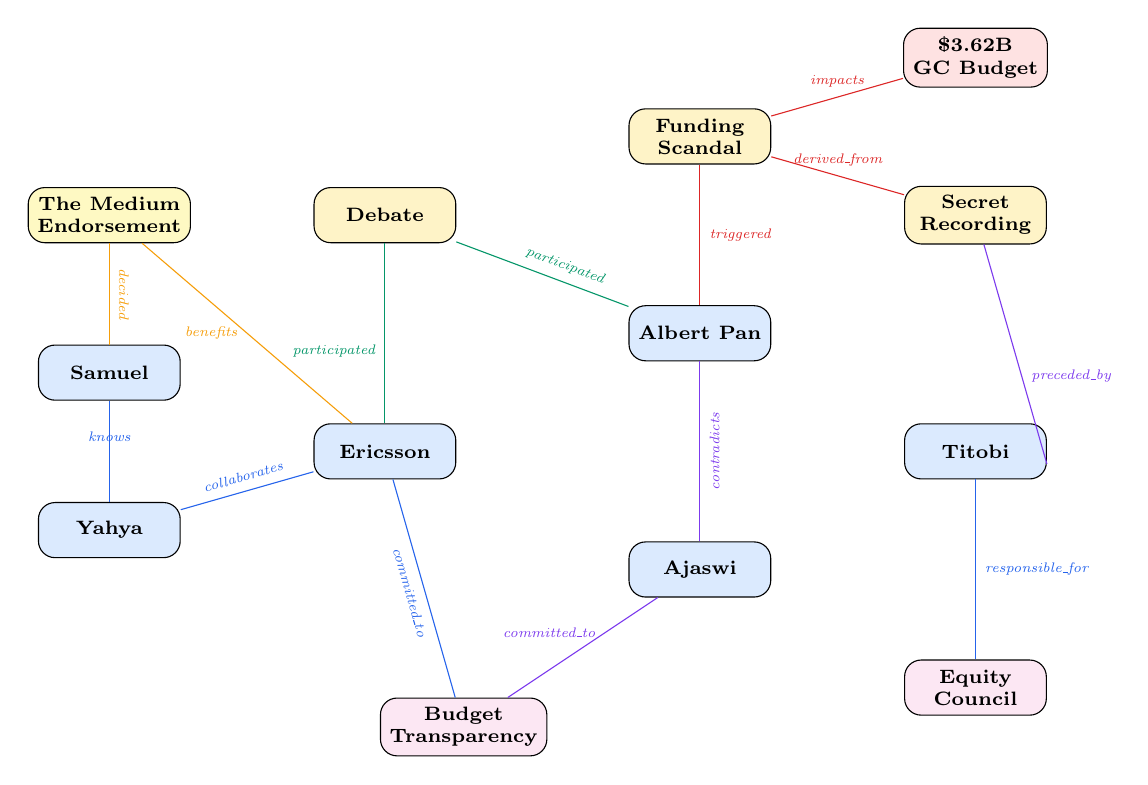
\begin{tikzpicture}[
    >={Stealth[length=4pt]},
    every edge/.style={draw, thick, ->},
    gnode/.style={draw, rounded corners=6pt, minimum width=1.8cm, minimum height=0.7cm, align=center, font=\scriptsize\bfseries, fill=#1},
]
    % People
    \node[gnode=nodeperson] (me) at (0, 0) {Ericsson};
    \node[gnode=nodeperson] (pan) at (4, 1.5) {Albert Pan};
    \node[gnode=nodeperson] (ajaswi) at (4, -1.5) {Ajaswi};
    \node[gnode=nodeperson] (yahya) at (-3.5, -1) {Yahya};
    \node[gnode=nodeperson] (samuel) at (-3.5, 1) {Samuel};
    \node[gnode=nodeperson] (titobi) at (7.5, 0) {Titobi};

    % Events
    \node[gnode=nodeevent] (scandal) at (4, 4) {Funding\\Scandal};
    \node[gnode=nodeevent] (debate) at (0, 3) {Debate};
    \node[gnode=nodeevent] (recording) at (7.5, 3) {Secret\\Recording};

    % Commitments
    \node[gnode=nodecommit] (audit) at (1, -3.5) {Budget\\Transparency};
    \node[gnode=nodecommit] (equity) at (7.5, -3) {Equity\\Council};

    % Decision
    \node[gnode=nodedecision] (endorsement) at (-3.5, 3) {The Medium\\Endorsement};

    % Financial
    \node[gnode=nodeidea] (budget) at (7.5, 5) {\$3.62B\\GC Budget};

    % Edges
    \draw[accent] (me) -- node[above, font=\tiny\itshape, sloped] {collaborates} (yahya);
    \draw[accent] (samuel) -- node[above, font=\tiny\itshape] {knows} (yahya);
    \draw[accent4] (pan) -- node[right, font=\tiny\itshape] {triggered} (scandal);
    \draw[accent2] (ajaswi) -- node[below, font=\tiny\itshape, sloped] {contradicts} (pan);
    \draw[accent3] (me) -- node[left, font=\tiny\itshape, pos=0.4] {participated} (debate);
    \draw[accent3] (pan) -- node[above, font=\tiny\itshape, sloped, pos=0.4] {participated} (debate);
    \draw[accent4] (recording) -- node[above, font=\tiny\itshape] {derived\_from} (scandal);
    \draw[accent] (titobi) -- node[right, font=\tiny\itshape] {responsible\_for} (equity);
    \draw[accent2] (ajaswi) -- node[left, font=\tiny\itshape, pos=0.35] {committed\_to} (audit);
    \draw[accent] (me) -- node[below, font=\tiny\itshape, sloped] {committed\_to} (audit);
    \draw[warm] (endorsement) -- node[above, font=\tiny\itshape, sloped] {decided} (samuel);
    \draw[warm] (endorsement) -- node[left, font=\tiny\itshape] {benefits} (me);
    \draw[accent4] (scandal) -- node[above, font=\tiny\itshape] {impacts} (budget);
    \draw[accent2] (recording) -- node[right, font=\tiny\itshape, pos=0.6] {preceded\_by} (titobi.-10);
\end{tikzpicture}%
}
\end{center}

Now you can traverse: start at Pan, follow \textsc{triggered} to the scandal, follow \textsc{derived\_from} to the recording, follow \textsc{preceded\_by} to see how Titobi cut ties. That's a story the graph tells through its structure---no keyword search required.

\begin{intuition}
The motivation is simple: life generates an overwhelming stream of interconnected information. Text files store it but can't reason about it. A knowledge graph preserves the \textbf{relationships} between things, and relationships are where the interesting answers live.
\end{intuition}

%==============================================================
\section{What Is Memora?}
%==============================================================

Memora is a personal decision intelligence system. You feed it unstructured text---notes, updates, stream-of-consciousness---and it produces a living knowledge graph that you can query, traverse, and that maintains itself over time.

The system rests on three ideas, each mapping to a course you've already taken:

\begin{center}
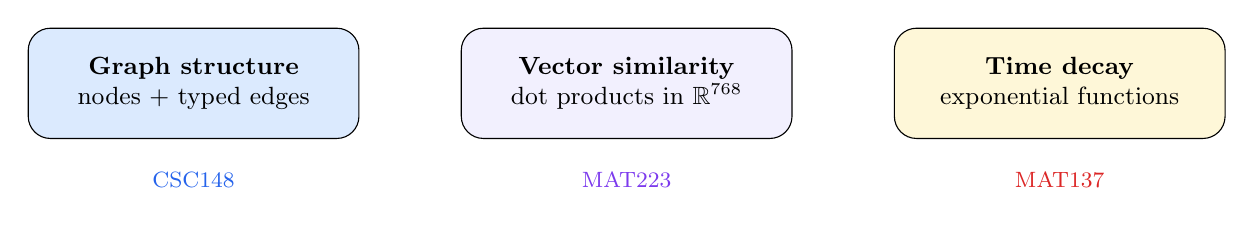
\begin{tikzpicture}[
    concept/.style={draw, rounded corners=8pt, fill=#1, minimum width=4.2cm, minimum height=1.4cm, align=center, font=\small},
]
    \node[concept=nodeperson] (g) at (0, 0) {\textbf{Graph structure}\\nodes + typed edges};
    \node[concept=nodenote!70] (v) at (5.5, 0) {\textbf{Vector similarity}\\dot products in $\mathbb{R}^{768}$};
    \node[concept=nodeevent!70] (d) at (11, 0) {\textbf{Time decay}\\exponential functions};

    \node[font=\footnotesize\color{accent}, below=0.3cm of g] {CSC148};
    \node[font=\footnotesize\color{accent2}, below=0.3cm of v] {MAT223};
    \node[font=\footnotesize\color{accent4}, below=0.3cm of d] {MAT137};
\end{tikzpicture}
\end{center}

Everything else---the pipeline, the agents, the background jobs---is iteration on this core.

%==============================================================
\section{The Graph --- CSC148 Thinking}
%==============================================================

Imagine you type this sentence into the system:

\begin{center}
\textit{``Had coffee with Sam. He'll intro me to his investor by Friday.\\Need to emphasize graph differentiation in the pitch deck.''}
\end{center}

Buried in that sentence are \textbf{five} distinct pieces of knowledge: an event (the coffee meeting), a person (Sam), a commitment (the investor intro), a note (the pitch strategy), and a project (the pitch deck). A traditional note-taking app stores this as flat text. You can search for keywords, but the app has no understanding of what ``Sam'' is, that there's a deadline, or that the pitch note relates to a project.

A \textbf{knowledge graph} does understand. It pulls apart the sentence into typed entities, connects them with named relationships, and creates a structure the computer can traverse, query, and reason about.

\begin{center}
\resizebox{0.85\textwidth}{!}{%
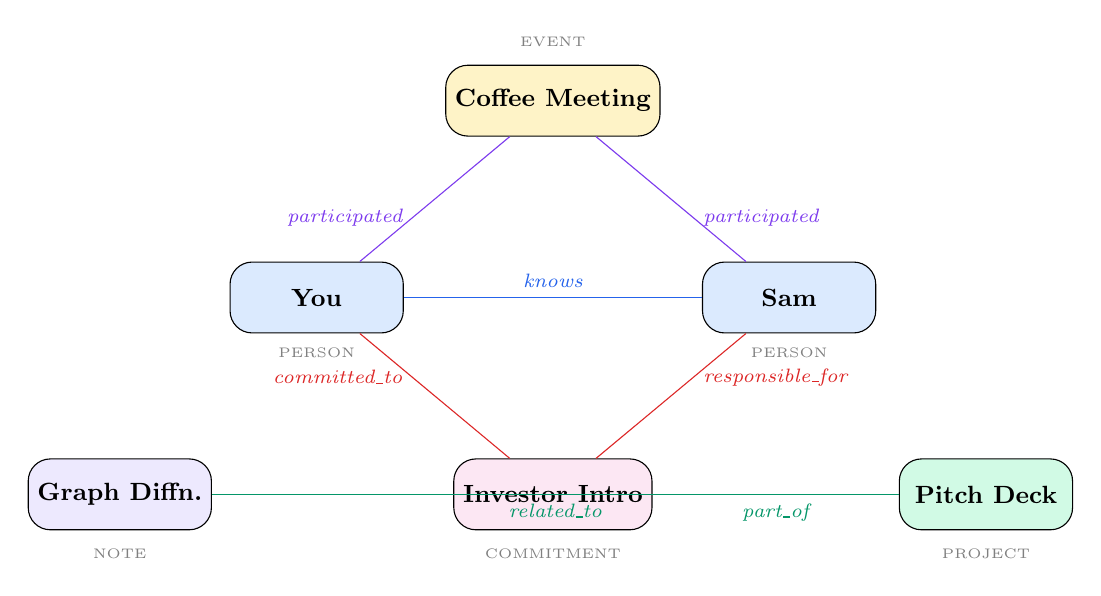
\begin{tikzpicture}[
    >={Stealth[length=5pt]},
    every edge/.style={draw, thick, ->},
    gnode/.style={draw, rounded corners=8pt, fill=#1, minimum width=2.2cm, minimum height=0.9cm, align=center, font=\small\bfseries},
]
    \node[gnode=nodeperson] (you) at (0, 0) {You};
    \node[gnode=nodeperson] (sam) at (6, 0) {Sam};
    \node[gnode=nodeevent] (event) at (3, 2.5) {Coffee Meeting};
    \node[gnode=nodecommit] (commit) at (3, -2.5) {Investor Intro};
    \node[gnode=nodeproject] (project) at (8.5, -2.5) {Pitch Deck};
    \node[gnode=nodenote] (note) at (-2.5, -2.5) {Graph Diffn.};

    % Type labels
    \node[font=\tiny\color{gray}] at (0, -0.7) {PERSON};
    \node[font=\tiny\color{gray}] at (6, -0.7) {PERSON};
    \node[font=\tiny\color{gray}] at (3, 3.25) {EVENT};
    \node[font=\tiny\color{gray}] at (3, -3.25) {COMMITMENT};
    \node[font=\tiny\color{gray}] at (8.5, -3.25) {PROJECT};
    \node[font=\tiny\color{gray}] at (-2.5, -3.25) {NOTE};

    \draw[accent] (you) -- node[above, font=\scriptsize\itshape] {knows} (sam);
    \draw[accent2] (you) -- node[left, font=\scriptsize\itshape, pos=0.35] {participated} (event);
    \draw[accent2] (sam) -- node[right, font=\scriptsize\itshape, pos=0.35] {participated} (event);
    \draw[accent4] (you) -- node[left, font=\scriptsize\itshape, pos=0.35] {committed\_to} (commit);
    \draw[accent4] (sam) -- node[right, font=\scriptsize\itshape, pos=0.35] {responsible\_for} (commit);
    \draw[accent3] (note) -- node[below, font=\scriptsize\itshape] {related\_to} (project);
    \draw[accent3] (commit) -- node[below, font=\scriptsize\itshape] {part\_of} (project);
\end{tikzpicture}%
}
\end{center}

One sentence became six nodes and seven edges. Now the system can answer questions like ``What's due this Friday?'', ``Who have I met recently?'', or ``What's connected to my pitch deck?''---not by keyword search, but by \textbf{traversing the graph}.

\begin{intuition}
A knowledge graph is the generalisation of a tree from CSC148---nodes can have multiple parents, cycles are allowed, and every edge has a label describing the relationship. If you can implement a tree with \texttt{add\_node} and \texttt{get\_children}, you can build a knowledge graph.
\end{intuition}

%==============================================================
\section{Where Does the Graph Come From?}
%==============================================================

You don't build the graph by hand. An LLM reads your text and proposes structured output---``I think this sentence contains an EVENT called `Coffee Meeting' and a PERSON called `Sam'.'' The system then decides whether ``Sam'' is a new person or someone already in the graph (more on this in Section~\ref{sec:entity-res}), and commits the changes.

\begin{center}
\resizebox{\textwidth}{!}{%
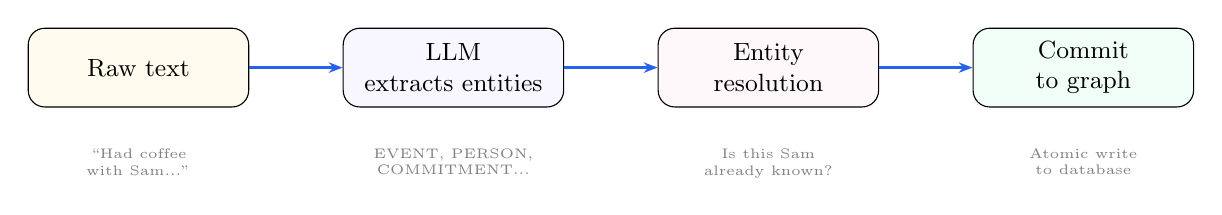
\begin{tikzpicture}[
    >={Stealth[length=5pt]},
    block/.style={draw, rounded corners=6pt, fill=#1, minimum width=2.8cm, minimum height=1cm, align=center, font=\small},
    arrow/.style={->, thick, accent},
]
    \node[block=nodeevent!30] (input) at (0, 0) {Raw text};
    \node[block=nodenote!40] (llm) at (4, 0) {LLM\\extracts entities};
    \node[block=nodecommit!30] (resolve) at (8, 0) {Entity\\resolution};
    \node[block=nodeproject!30] (commit) at (12, 0) {Commit\\to graph};

    \draw[arrow] (input) -- (llm);
    \draw[arrow] (llm) -- (resolve);
    \draw[arrow] (resolve) -- (commit);

    \node[below=0.4cm of input, font=\tiny\color{gray}, align=center] {``Had coffee\\with Sam...''};
    \node[below=0.4cm of llm, font=\tiny\color{gray}, align=center] {EVENT, PERSON,\\COMMITMENT...};
    \node[below=0.4cm of resolve, font=\tiny\color{gray}, align=center] {Is this Sam\\already known?};
    \node[below=0.4cm of commit, font=\tiny\color{gray}, align=center] {Atomic write\\to database};
\end{tikzpicture}%
}
\end{center}

The LLM is a tool, not the system. Remove it entirely and the graph mechanics---the decay, the search, the bridge discovery---all continue to work. But how the LLM does its job---reading English and producing structured data---is worth understanding. The next section explains what ``structured output'' actually means and how the system keeps the LLM on a short leash.

%==============================================================
\section{The Role of the LLM}
\label{sec:llm-role}
%==============================================================

When you type ``Titobi was negotiating to endorse Pan, then cut ties after a leaked recording,'' something has to decide that Titobi and Pan are people, that the endorsement negotiation is an event, and that a secret recording caused a relationship to break. That something is an LLM---but not the free-form chatbot you're used to. Here, the LLM operates as a \textbf{constrained function}: given structured input, it must produce structured output conforming to a strict schema. If it doesn't, we retry or discard.

\subsection{Three Layers of Constraint}

The system keeps the LLM on a short leash through three progressively narrower layers:

\begin{center}
\resizebox{0.92\textwidth}{!}{%
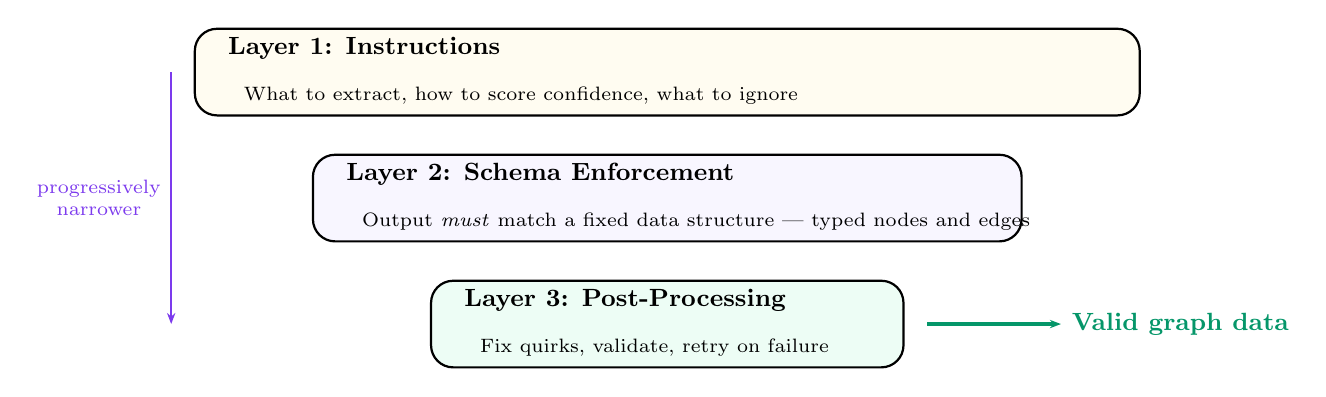
\begin{tikzpicture}[
    >={Stealth[length=4pt]},
    layer/.style={draw, rounded corners=8pt, thick, fill=#1, minimum height=1.1cm, align=center, font=\small},
]
    % Outermost layer
    \node[layer=nodeevent!25, minimum width=12cm] (l1) at (0, 2.4) {};
    \node[font=\small\bfseries, anchor=west] at (-5.7, 2.7) {Layer 1: Instructions};
    \node[font=\scriptsize, align=left, anchor=west] at (-5.5, 2.1) {What to extract, how to score confidence, what to ignore};

    % Middle layer
    \node[layer=nodenote!40, minimum width=9cm] (l2) at (0, 0.8) {};
    \node[font=\small\bfseries, anchor=west] at (-4.2, 1.1) {Layer 2: Schema Enforcement};
    \node[font=\scriptsize, align=left, anchor=west] at (-4.0, 0.5) {Output \emph{must} match a fixed data structure --- typed nodes and edges};

    % Innermost layer
    \node[layer=nodeproject!40, minimum width=6cm] (l3) at (0, -0.8) {};
    \node[font=\small\bfseries, anchor=west] at (-2.7, -0.5) {Layer 3: Post-Processing};
    \node[font=\scriptsize, align=left, anchor=west] at (-2.5, -1.1) {Fix quirks, validate, retry on failure};

    % Arrows showing narrowing
    \draw[->, thick, accent2] (-6.3, 2.4) -- (-6.3, -0.8) node[midway, left, font=\scriptsize\color{accent2}, align=center] {progressively\\narrower};

    % Output label
    \draw[->, very thick, accent3] (3.3, -0.8) -- (5, -0.8) node[right, font=\small\bfseries\color{accent3}] {Valid graph data};
\end{tikzpicture}%
}
\end{center}

Instructions tell the LLM \emph{what} to find. The schema tells it \emph{how} to format the answer. Post-processing catches anything it still gets wrong---malformed output, invented categories, scores out of range---and either fixes or retries.

\begin{intuition}
Think of it like defining a function in MAT137: you specify the domain (what goes in), the codomain (what comes out), and you verify the output is actually in the codomain before using it. The LLM might be a black box internally, but its \emph{interface} is fully specified.
\end{intuition}

\subsection{What Goes In, What Comes Out}

The LLM receives the raw text plus what the system already knows, and must produce typed graph elements:

\begin{center}
\resizebox{0.92\textwidth}{!}{%
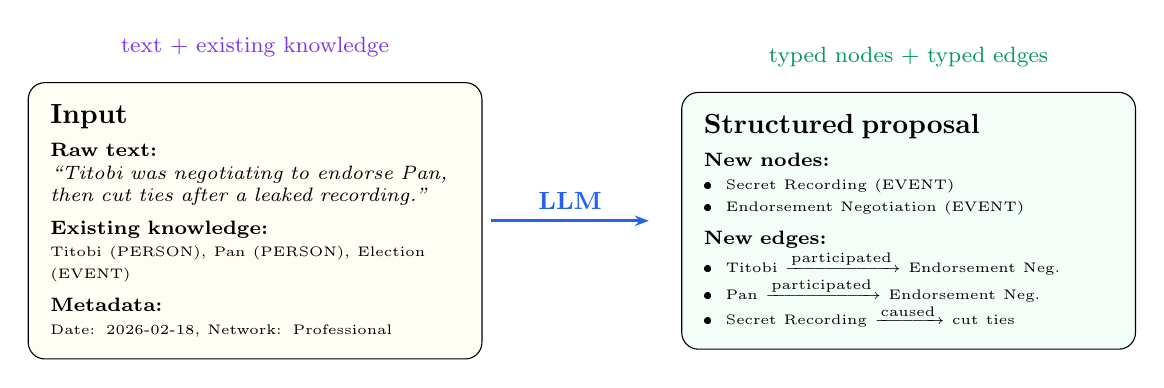
\begin{tikzpicture}[
    >={Stealth[length=5pt]},
    inbox/.style={draw, rounded corners=6pt, fill=#1, minimum width=5cm, align=left, font=\scriptsize, inner sep=8pt},
]
    % Input side
    \node[inbox=nodeevent!20, text width=5.2cm] (input) at (0, 0) {
        \textbf{\normalsize Input}\\[4pt]
        \textbf{Raw text:}\\
        \textit{``Titobi was negotiating to endorse Pan, then cut ties after a leaked recording.''}\\[4pt]
        \textbf{Existing knowledge:}\\
        {\tiny Titobi (PERSON), Pan (PERSON), Election (EVENT)}\\[4pt]
        \textbf{Metadata:}\\
        {\tiny Date: 2026-02-18, Network: Professional}
    };

    % Arrow
    \draw[->, very thick, accent] (3.0, 0) -- node[above, font=\small\bfseries] {LLM} (5.0, 0);

    % Output side
    \node[inbox=nodeproject!25, text width=5.2cm] (output) at (8.3, 0) {
        \textbf{\normalsize Structured proposal}\\[4pt]
        \textbf{New nodes:}\\
        {\tiny \textbullet\; Secret Recording (EVENT)}\\
        {\tiny \textbullet\; Endorsement Negotiation (EVENT)}\\[4pt]
        \textbf{New edges:}\\
        {\tiny \textbullet\; Titobi $\xrightarrow{\text{participated}}$ Endorsement Neg.}\\
        {\tiny \textbullet\; Pan $\xrightarrow{\text{participated}}$ Endorsement Neg.}\\
        {\tiny \textbullet\; Secret Recording $\xrightarrow{\text{caused}}$ cut ties}
    };

    % Labels
    \node[font=\footnotesize\color{accent2}, above=0.2cm of input] {text + existing knowledge};
    \node[font=\footnotesize\color{accent3}, above=0.2cm of output] {typed nodes + typed edges};
\end{tikzpicture}%
}
\end{center}

The LLM doesn't produce prose---it produces typed nodes and edges. Because the system already has Titobi and Pan in the graph, it tells the LLM ``these people exist; reference them, don't re-create them.''

\subsection{Multiple Specialists, Not One Oracle}

Rather than one LLM doing everything, the system uses \textbf{three specialist agents}:

\begin{center}
\resizebox{0.92\textwidth}{!}{%
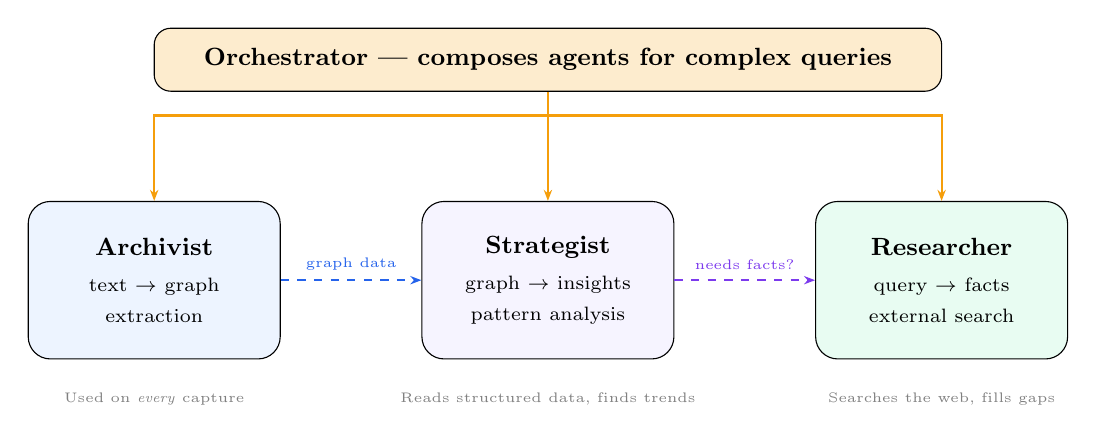
\begin{tikzpicture}[
    >={Stealth[length=4pt]},
    agent/.style={draw, rounded corners=8pt, fill=#1, minimum width=3.2cm, minimum height=2cm, align=center, font=\small},
    domainlabel/.style={font=\tiny\color{gray}, align=center},
]
    % Archivist
    \node[agent=nodeperson!50] (arch) at (0, 0) {\textbf{Archivist}\\[2pt]{\scriptsize text $\to$ graph}\\{\scriptsize extraction}};
    \node[domainlabel, below=0.3cm of arch] {Used on \emph{every} capture};

    % Strategist
    \node[agent=nodenote!50] (strat) at (5, 0) {\textbf{Strategist}\\[2pt]{\scriptsize graph $\to$ insights}\\{\scriptsize pattern analysis}};
    \node[domainlabel, below=0.3cm of strat] {Reads structured data, finds trends};

    % Researcher
    \node[agent=nodeproject!50] (res) at (10, 0) {\textbf{Researcher}\\[2pt]{\scriptsize query $\to$ facts}\\{\scriptsize external search}};
    \node[domainlabel, below=0.3cm of res] {Searches the web, fills gaps};

    % Orchestrator
    \node[draw, rounded corners=6pt, fill=warm!20, minimum width=10cm, minimum height=0.8cm, font=\small\bfseries] (orch) at (5, 2.8) {Orchestrator --- composes agents for complex queries};

    % Connections from orchestrator
    \draw[->, thick, warm] (orch.south) -- ++(0, -0.3) -| (arch.north);
    \draw[->, thick, warm] (orch.south) -- ++(0, -0.3) -| (strat.north);
    \draw[->, thick, warm] (orch.south) -- ++(0, -0.3) -| (res.north);

    % Flow arrows between agents
    \draw[->, thick, accent, dashed] (arch.east) -- node[above, font=\tiny] {graph data} (strat.west);
    \draw[->, thick, accent2, dashed] (strat.east) -- node[above, font=\tiny] {needs facts?} (res.west);
\end{tikzpicture}%
}
\end{center}

Each specialist stays in its lane---the Archivist never analyses patterns, the Strategist never parses raw text. The Orchestrator is function composition: when you ask ``What patterns connect my academic and professional networks?'', it chains the right specialists together.

\begin{keyidea}
The LLM is powerful but unreliable. The system constrains it---defines inputs and outputs precisely, validates everything it produces, and splits complex work across specialists with narrow responsibilities.
\end{keyidea}

%==============================================================
\section{Making the Computer Understand ``Similar''}
\label{sec:vectors}
%==============================================================

Here is the central question: you have two pieces of text. How does a computer know they're about the same thing?

\subsection{Turning Words Into Arrows}

A pretrained model acts as a function $f$ that maps any sentence to a point in 768-dimensional space:
\[
    f(\text{``Discussed pitch strategy with Sam''}) \;\longrightarrow\; \text{a point in } \mathbb{R}^{768}
\]

You don't build $f$---you download it. The key property it was trained to have: \textbf{sentences with similar meaning land near each other}.

We can visualise this by projecting down to 2D. Even though ``Had coffee with Sam to discuss the pitch'' contains the word ``coffee,'' its vector lands near the pitch cluster, not the coffee cluster. The model captures \emph{meaning}, not keywords.

\begin{center}
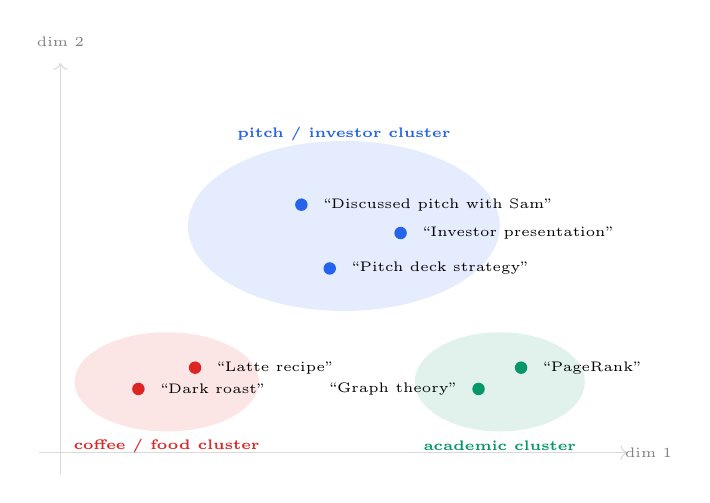
\begin{tikzpicture}[scale=0.9]
    % Axes
    \draw[gray!30, ->] (-0.3,0) -- (8,0);
    \draw[gray!30, ->] (0,-0.3) -- (0,5.5);
    \node[font=\tiny\color{gray}] at (8.3,0) {dim 1};
    \node[font=\tiny\color{gray}] at (0,5.8) {dim 2};

    % Cluster 1: pitch-related
    \fill[accent!12, rounded corners=10pt] (4,3.2) ellipse (2.2cm and 1.2cm);
    \node[font=\tiny\bfseries\color{accent}] at (4,4.5) {pitch / investor cluster};
    \fill[accent] (3.4,3.5) circle (2.5pt);
    \node[font=\tiny, right] at (3.55,3.5) {``Discussed pitch with Sam''};
    \fill[accent] (4.8,3.1) circle (2.5pt);
    \node[font=\tiny, right] at (4.95,3.1) {``Investor presentation''};
    \fill[accent] (3.8,2.6) circle (2.5pt);
    \node[font=\tiny, right] at (3.95,2.6) {``Pitch deck strategy''};

    % Cluster 2: coffee-unrelated
    \fill[accent4!12, rounded corners=10pt] (1.5,1) ellipse (1.3cm and 0.7cm);
    \node[font=\tiny\bfseries\color{accent4}] at (1.5,0.1) {coffee / food cluster};
    \fill[accent4] (1.1,0.9) circle (2.5pt);
    \node[font=\tiny, right] at (1.25,0.9) {``Dark roast''};
    \fill[accent4] (1.9,1.2) circle (2.5pt);
    \node[font=\tiny, right] at (2.05,1.2) {``Latte recipe''};

    % Cluster 3: academic
    \fill[accent3!12, rounded corners=10pt] (6.2,1) ellipse (1.2cm and 0.7cm);
    \node[font=\tiny\bfseries\color{accent3}] at (6.2,0.1) {academic cluster};
    \fill[accent3] (5.9,0.9) circle (2.5pt);
    \node[font=\tiny, left] at (5.75,0.9) {``Graph theory''};
    \fill[accent3] (6.5,1.2) circle (2.5pt);
    \node[font=\tiny, right] at (6.65,1.2) {``PageRank''};
\end{tikzpicture}
\end{center}

\subsection{Measuring Closeness: The Dot Product You Already Know}

In MAT223 you learned that the dot product encodes the angle between two vectors:
\[
    \langle \mathbf{u}, \mathbf{v} \rangle \;=\; \|\mathbf{u}\|\;\|\mathbf{v}\|\;\cos\theta
\]

Rearrange to isolate the angle, and you get \textbf{cosine similarity}:
\[
    \cos\theta \;=\; \frac{\langle \mathbf{u}, \mathbf{v} \rangle}{\|\mathbf{u}\|\;\|\mathbf{v}\|}
\]

\begin{center}
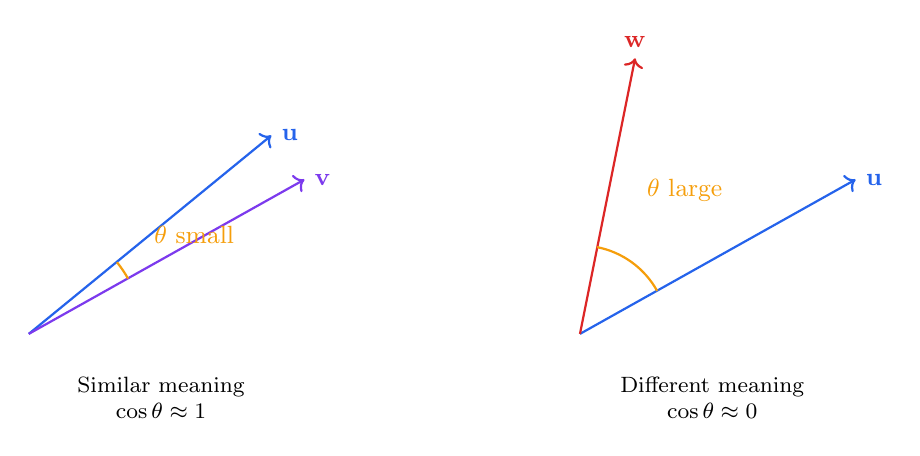
\begin{tikzpicture}[scale=1.4]
    % Similar pair
    \begin{scope}
        \draw[->, thick, accent] (0,0) -- (2.2,1.8) node[right, font=\small] {$\mathbf{u}$};
        \draw[->, thick, accent2] (0,0) -- (2.5,1.4) node[right, font=\small] {$\mathbf{v}$};
        \draw[thick, warm] (0.8,0.65) arc[start angle=39, end angle=29, radius=1.03];
        \node[font=\small, warm] at (1.5, 0.9) {$\theta$ small};
        \node[below, font=\footnotesize, align=center] at (1.2,-0.3) {Similar meaning\\$\cos\theta \approx 1$};
    \end{scope}
    % Dissimilar pair
    \begin{scope}[xshift=5cm]
        \draw[->, thick, accent] (0,0) -- (2.5,1.4) node[right, font=\small] {$\mathbf{u}$};
        \draw[->, thick, accent4] (0,0) -- (0.5,2.5) node[above, font=\small] {$\mathbf{w}$};
        \draw[thick, warm] (0.7,0.39) arc[start angle=29, end angle=79, radius=0.8];
        \node[font=\small, warm] at (0.95, 1.3) {$\theta$ large};
        \node[below, font=\footnotesize, align=center] at (1.2,-0.3) {Different meaning\\$\cos\theta \approx 0$};
    \end{scope}
\end{tikzpicture}
\end{center}

\begin{keyidea}
\textbf{Cosine similarity is the entire foundation of semantic search.} To find nodes related to a query, embed the query as a vector, compute the cosine angle against every stored node, and return the closest ones. It's the MAT223 dot product---in 768 dimensions instead of 3.
\end{keyidea}

The intuition scales perfectly: inner products, norms, and angles obey the same axioms in $\mathbb{R}^{768}$ as in $\mathbb{R}^2$. You just can't draw it on a whiteboard. Think of each of the 768 dimensions as one axis of meaning---the same way basis vectors $\mathbf{e}_1, \dots, \mathbf{e}_n$ span $\mathbb{R}^n$.

%==============================================================
\section{``Is This the Same Sam?'' --- Entity Resolution}
\label{sec:entity-res}
%==============================================================

Every time the LLM extracts a person, event, or idea, the system must decide: is this something \textbf{new}, or does it already exist in the graph? Getting this wrong means duplicates everywhere.

The answer is another linear algebra idea. Collect multiple signals about the candidate match, stack them as a vector, and take a weighted dot product:

\begin{center}
\resizebox{0.95\textwidth}{!}{%
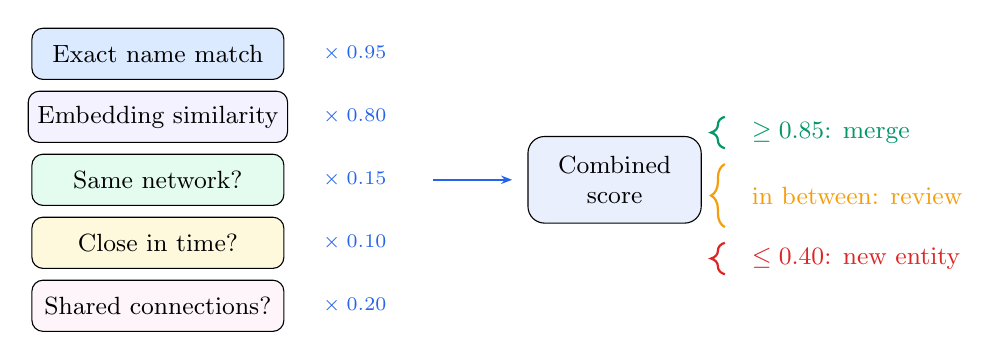
\begin{tikzpicture}[
    signal/.style={draw, rounded corners=4pt, fill=#1, minimum width=3.2cm, minimum height=0.65cm, align=center, font=\small},
    >={Stealth[length=4pt]},
]
    % Signal bars
    \node[signal=nodeperson] (s1) at (0, 2.6) {Exact name match};
    \node[signal=nodenote!60] (s2) at (0, 1.8) {Embedding similarity};
    \node[signal=nodeproject!60] (s3) at (0, 1.0) {Same network?};
    \node[signal=nodeevent!60] (s4) at (0, 0.2) {Close in time?};
    \node[signal=nodecommit!40] (s5) at (0, -0.6) {Shared connections?};

    % Weight labels
    \node[font=\scriptsize\bfseries\color{accent}] at (2.5, 2.6) {$\times\; 0.95$};
    \node[font=\scriptsize\bfseries\color{accent}] at (2.5, 1.8) {$\times\; 0.80$};
    \node[font=\scriptsize\bfseries\color{accent}] at (2.5, 1.0) {$\times\; 0.15$};
    \node[font=\scriptsize\bfseries\color{accent}] at (2.5, 0.2) {$\times\; 0.10$};
    \node[font=\scriptsize\bfseries\color{accent}] at (2.5, -0.6) {$\times\; 0.20$};

    % Arrow to score
    \draw[->, thick, accent] (3.5, 1.0) -- (4.5, 1.0);

    % Score box
    \node[draw, rounded corners=6pt, fill=accent!10, minimum width=2.2cm, minimum height=1.1cm, align=center, font=\small] (score) at (5.8, 1.0) {Combined\\score};

    % Decision zones
    \draw[decorate, decoration={brace, amplitude=5pt, mirror}, thick, accent3] (7.2, 1.8) -- (7.2, 1.4) node[midway, right=6pt, font=\small\color{accent3}] {$\geq 0.85$: merge};
    \draw[decorate, decoration={brace, amplitude=5pt, mirror}, thick, warm] (7.2, 1.2) -- (7.2, 0.4) node[midway, right=6pt, font=\small\color{warm}] {in between: review};
    \draw[decorate, decoration={brace, amplitude=5pt, mirror}, thick, accent4] (7.2, 0.2) -- (7.2, -0.2) node[midway, right=6pt, font=\small\color{accent4}] {$\leq 0.40$: new entity};
\end{tikzpicture}%
}
\end{center}

This is exactly a \textbf{linear combination}---a weight vector $\mathbf{w}$ dotted with a signal vector $\mathbf{s}$:
\[
    \text{score} = \langle \mathbf{w},\, \mathbf{s} \rangle
\]

The threshold $\langle \mathbf{w}, \mathbf{s} \rangle = 0.85$ is a hyperplane in signal space, cutting the space into a ``merge'' half and a ``don't merge'' half---the same geometric picture of half-spaces from MAT223.

\begin{intuition}
Entity resolution is not magic. It's asking ``how similar is this candidate on multiple axes?'' and collapsing those axes into a single number via a dot product. You've been doing this since MAT223.
\end{intuition}

%==============================================================
\section{The Graph Stays Alive: Decay}
%==============================================================

A static graph becomes useless fast. During the election, Capture 6 (campaign dirty tricks) was urgent on the day it happened. Two weeks later, Capture 14 (building the administration) matters far more. The system needs a notion of \textbf{relevance over time}.

\subsection{The Decay Curve}

Every node carries a score that fades with time:
\[
    \text{score}(t) = e^{-\lambda t}
\]

You know this function from MAT137. Different knowledge domains decay at different rates---a social interaction gets stale in ten days, but a financial commitment stays relevant for over a month:

\begin{center}
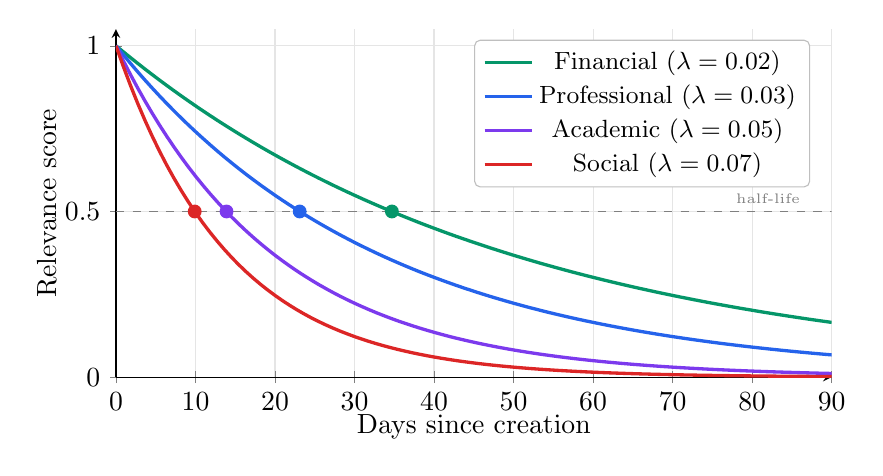
\begin{tikzpicture}
\begin{axis}[
    width=0.88\textwidth, height=6cm,
    xlabel={Days since creation},
    ylabel={Relevance score},
    xmin=0, xmax=90,
    ymin=0, ymax=1.05,
    grid=major,
    grid style={gray!20},
    legend style={at={(0.97,0.97)}, anchor=north east, font=\small, draw=gray!50, fill=white, rounded corners=2pt},
    axis lines=left,
    every axis x label/.style={at={(axis description cs:0.5,-0.08)}, anchor=north},
    every axis y label/.style={at={(axis description cs:-0.07,0.5)}, rotate=90, anchor=south},
]
    \addplot[accent3, very thick, domain=0:90, samples=100] {exp(-0.02*x)};
    \addlegendentry{Financial ($\lambda = 0.02$)}

    \addplot[accent, very thick, domain=0:90, samples=100] {exp(-0.03*x)};
    \addlegendentry{Professional ($\lambda = 0.03$)}

    \addplot[accent2, very thick, domain=0:90, samples=100] {exp(-0.05*x)};
    \addlegendentry{Academic ($\lambda = 0.05$)}

    \addplot[accent4, very thick, domain=0:90, samples=100] {exp(-0.07*x)};
    \addlegendentry{Social ($\lambda = 0.07$)}

    % Half-life line
    \addplot[dashed, gray, thin] coordinates {(0,0.5) (90,0.5)};
    \node[font=\tiny\color{gray}] at (axis cs:82,0.54) {half-life};

    % Half-life dots
    \fill[accent4] (axis cs:9.9,0.5) circle (2.5pt);
    \fill[accent2] (axis cs:13.9,0.5) circle (2.5pt);
    \fill[accent] (axis cs:23.1,0.5) circle (2.5pt);
    \fill[accent3] (axis cs:34.7,0.5) circle (2.5pt);
\end{axis}
\end{tikzpicture}
\end{center}

The \textbf{half-life}---the time for a node's score to drop to 50\%---is $t_{1/2} = \ln 2 / \lambda$:

\begin{center}
\renewcommand{\arraystretch}{1.3}
\begin{tabular}{l c c l}
    \hline
    \textbf{Network} & \boldmath$\lambda$ & \textbf{Half-life} & \textbf{Intuition} \\
    \hline
    Financial    & 0.02 & $\sim\!35$ days & Tax deadlines, the \$3.62B budget question lingers \\
    Professional & 0.03 & $\sim\!23$ days & Committee roles, endorsements stay relevant for weeks \\
    Academic     & 0.05 & $\sim\!14$ days & Course material, debate arguments cycle faster \\
    Social       & 0.07 & $\sim\!10$ days & ``We should hang out'' expires quickly \\
    \hline
\end{tabular}
\end{center}

\subsection{Why This Shape?}

The properties of $e^{-\lambda t}$ are exactly what you want for modelling memory:

\begin{center}
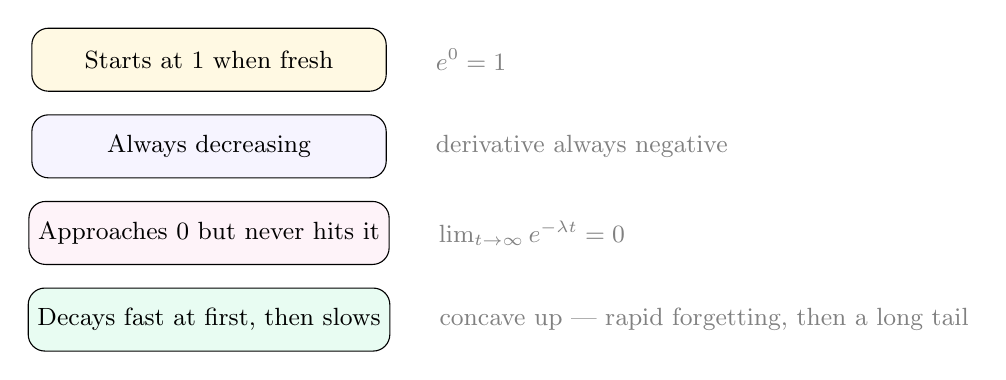
\begin{tikzpicture}[
    prop/.style={draw, rounded corners=6pt, fill=#1, minimum width=4.5cm, minimum height=0.8cm, align=center, font=\small},
]
    \node[prop=nodeevent!50] (p1) at (0, 2.2) {Starts at $1$ when fresh};
    \node[prop=nodenote!50] (p2) at (0, 1.1) {Always decreasing};
    \node[prop=nodecommit!50] (p3) at (0, 0.0) {Approaches $0$ but never hits it};
    \node[prop=nodeproject!50] (p4) at (0, -1.1) {Decays fast at first, then slows};

    \node[font=\small\color{gray}, right=0.5cm of p1] {$e^{0} = 1$};
    \node[font=\small\color{gray}, right=0.5cm of p2] {derivative always negative};
    \node[font=\small\color{gray}, right=0.5cm of p3] {$\lim_{t\to\infty} e^{-\lambda t} = 0$};
    \node[font=\small\color{gray}, right=0.5cm of p4] {concave up --- rapid forgetting, then a long tail};
\end{tikzpicture}
\end{center}

That last property---concavity---is the interesting one. A one-week-old note loses relevance quickly. But a six-month-old note that's still around barely changes from one day to the next. This mirrors how human memory actually works.

\subsection{The More You Look, The Slower It Fades}

If you keep accessing a node, it should decay more slowly. The system modulates the decay rate with a logarithmic damper:
\[
    \lambda_{\text{eff}} = \frac{\lambda}{1 + \ln(1 + n)}
\]
where $n$ is how many times you've accessed the node.

\begin{center}
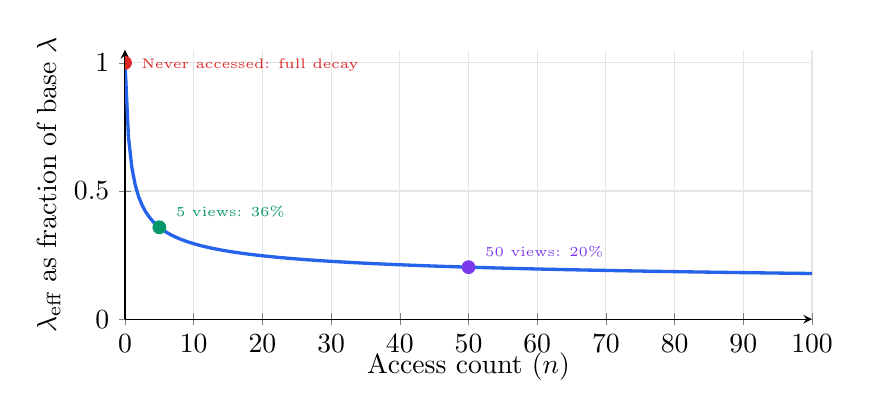
\begin{tikzpicture}
\begin{axis}[
    width=0.85\textwidth, height=5cm,
    xlabel={Access count ($n$)},
    ylabel={$\lambda_{\text{eff}}$ as fraction of base $\lambda$},
    xmin=0, xmax=100,
    ymin=0, ymax=1.05,
    grid=major,
    grid style={gray!20},
    axis lines=left,
    every axis x label/.style={at={(axis description cs:0.5,-0.09)}, anchor=north},
    every axis y label/.style={at={(axis description cs:-0.08,0.5)}, rotate=90, anchor=south},
]
    \addplot[accent, very thick, domain=0:100, samples=200] {1/(1 + ln(1+x))};

    \fill[accent4] (axis cs:0,1) circle (2.5pt);
    \node[font=\tiny, accent4, above right] at (axis cs:1,0.93) {Never accessed: full decay};

    \fill[accent3] (axis cs:5,{1/(1+ln(6))}) circle (2.5pt);
    \node[font=\tiny, accent3, above right] at (axis cs:6,{1/(1+ln(6))}) {5 views: 36\%};

    \fill[accent2] (axis cs:50,{1/(1+ln(51))}) circle (2.5pt);
    \node[font=\tiny, accent2, above right] at (axis cs:51,{1/(1+ln(51))}) {50 views: 20\%};
\end{axis}
\end{tikzpicture}
\end{center}

From MAT137 you know $\ln$ grows slower than any polynomial---so the first few accesses matter a lot, but the 100th barely differs from the 99th. A node you accidentally click 500 times won't become immortal, but one you genuinely keep returning to will persist.

%==============================================================
\section{Discovering Hidden Connections}
%==============================================================

The most interesting thing a knowledge graph can do is find connections \emph{you didn't explicitly make}.

In the election scenario, your Academic network has nodes about governance structures and committee processes. Your Ventures network, separately, has nodes about accountability dashboards and data transparency. You never connected them---but their embedding vectors point in nearly the same direction. The system finds this bridge automatically.

\begin{center}
\resizebox{0.92\textwidth}{!}{%
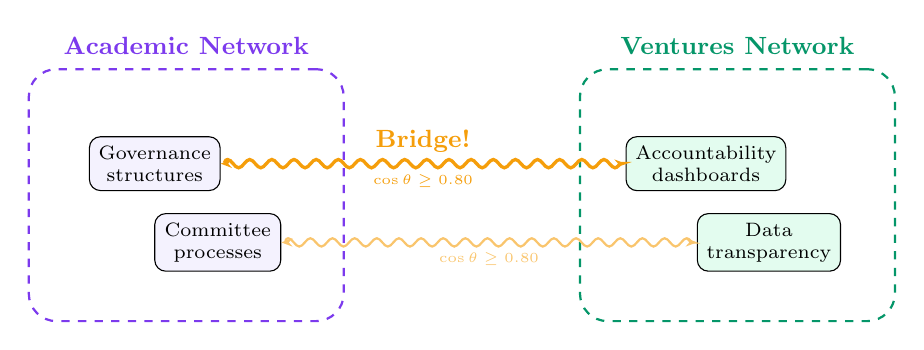
\begin{tikzpicture}[
    >={Stealth[length=4pt]},
    netbox/.style={draw, rounded corners=10pt, dashed, thick, minimum width=4cm, minimum height=3.2cm, #1},
    inner/.style={draw, rounded corners=4pt, fill=#1, font=\scriptsize, align=center, minimum width=1.6cm, minimum height=0.6cm},
]
    % Academic network
    \node[netbox=accent2] (acad) at (0,0) {};
    \node[font=\small\bfseries\color{accent2}] at (0, 1.9) {Academic Network};
    \node[inner=nodenote!60] (c1) at (-0.4, 0.4) {Governance\\structures};
    \node[inner=nodenote!60] (c2) at (0.4, -0.6) {Committee\\processes};

    % Ventures network
    \node[netbox=accent3] (vent) at (7,0) {};
    \node[font=\small\bfseries\color{accent3}] at (7, 1.9) {Ventures Network};
    \node[inner=nodeproject!60] (p1) at (6.6, 0.4) {Accountability\\dashboards};
    \node[inner=nodeproject!60] (p2) at (7.4, -0.6) {Data\\transparency};

    % Bridges
    \draw[<->, very thick, warm, decorate, decoration={snake, amplitude=1.5pt, segment length=8pt}]
        (c1.east) -- node[above, font=\small\bfseries\color{warm}] {Bridge!}
                     node[below, font=\tiny\color{gray}] {$\cos\theta \geq 0.80$} (p1.west);
    \draw[<->, thick, warm!60, decorate, decoration={snake, amplitude=1.5pt, segment length=8pt}]
        (c2.east) -- node[below, font=\tiny\color{gray}] {$\cos\theta \geq 0.80$} (p2.west);
\end{tikzpicture}%
}
\end{center}

In MAT223 terms: you're looking for vector pairs from different subsets of $\mathbb{R}^{768}$ whose angle $\theta$ satisfies $\cos\theta \geq 0.80$, meaning $\theta \leq 37°$. Nearly parallel vectors from different life domains signal a hidden insight.

%==============================================================
\section{Spaced Repetition: When to Resurface Knowledge}
%==============================================================

Some nodes shouldn't just decay---they should be \textbf{actively reviewed}. The system uses a classic spacing algorithm where review intervals form a geometric sequence:

\begin{center}
\resizebox{0.92\textwidth}{!}{%
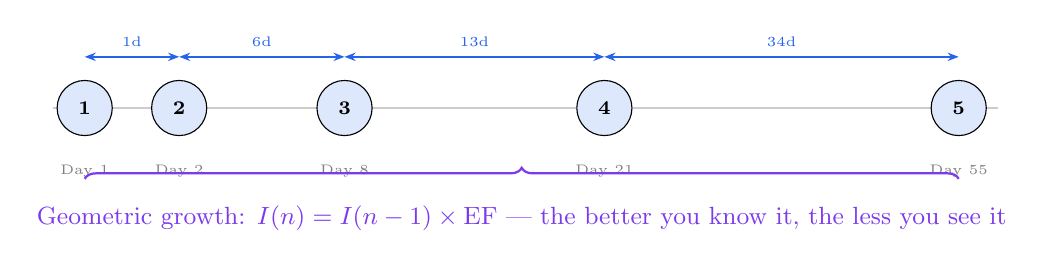
\begin{tikzpicture}[
    >={Stealth[length=4pt]},
    review/.style={draw, circle, fill=accent!15, minimum size=0.7cm, font=\scriptsize\bfseries, inner sep=0pt},
]
    % Timeline
    \draw[thick, gray!40] (0,0) -- (12,0);

    % Review points
    \node[review] (r1) at (0.4,0) {1};
    \node[review] (r2) at (1.6,0) {2};
    \node[review] (r3) at (3.7,0) {3};
    \node[review] (r4) at (7,0) {4};
    \node[review] (r5) at (11.5,0) {5};

    % Day labels
    \node[below=0.25cm of r1, font=\tiny\color{gray}] {Day 1};
    \node[below=0.25cm of r2, font=\tiny\color{gray}] {Day 2};
    \node[below=0.25cm of r3, font=\tiny\color{gray}] {Day 8};
    \node[below=0.25cm of r4, font=\tiny\color{gray}] {Day 21};
    \node[below=0.25cm of r5, font=\tiny\color{gray}] {Day 55};

    % Interval annotations
    \draw[<->, thick, accent] (0.4,0.65) -- node[above, font=\tiny] {1d} (1.6,0.65);
    \draw[<->, thick, accent] (1.6,0.65) -- node[above, font=\tiny] {6d} (3.7,0.65);
    \draw[<->, thick, accent] (3.7,0.65) -- node[above, font=\tiny] {13d} (7,0.65);
    \draw[<->, thick, accent] (7,0.65) -- node[above, font=\tiny] {34d} (11.5,0.65);

    % Growth annotation
    \draw[decorate, decoration={brace, amplitude=4pt}, thick, accent2] (0.4,-0.9) -- (11.5,-0.9)
        node[midway, below=6pt, font=\small\color{accent2}, align=center]
        {Geometric growth: $I(n) = I(n-1) \times \text{EF}$ --- the better you know it, the less you see it};
\end{tikzpicture}%
}
\end{center}

This is a geometric sequence with ratio $\text{EF} \geq 1.3$. From MAT137 you know this diverges---the gaps grow without bound, which is exactly what you want. Things you remember well eventually stop appearing.

%==============================================================
\section{Two-Layer Storage}
%==============================================================

All of this needs to be stored somewhere. The system uses two complementary databases---one for structure, one for meaning:

\begin{center}
\resizebox{0.92\textwidth}{!}{%
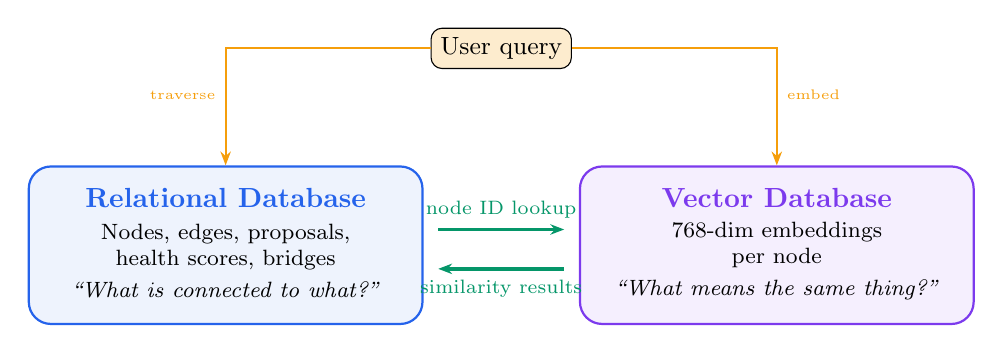
\begin{tikzpicture}[
    >={Stealth[length=5pt]},
    layer/.style={draw, rounded corners=8pt, thick, minimum width=5cm, minimum height=2cm, align=center, #1},
]
    % DuckDB
    \node[layer={fill=accent!8, draw=accent}] (duck) at (0, 0) {};
    \node[font=\bfseries\color{accent}] at (0, 0.6) {Relational Database};
    \node[font=\footnotesize, align=center] at (0, -0.2) {Nodes, edges, proposals,\\health scores, bridges\\[2pt]\textit{``What is connected to what?''}};

    % Weaviate
    \node[layer={fill=accent2!8, draw=accent2}] (weav) at (7, 0) {};
    \node[font=\bfseries\color{accent2}] at (7, 0.6) {Vector Database};
    \node[font=\footnotesize, align=center] at (7, -0.2) {768-dim embeddings\\per node\\[2pt]\textit{``What means the same thing?''}};

    % Arrows between
    \draw[->, very thick, accent3] (2.7, 0.2) -- node[above, font=\scriptsize] {node ID lookup} (4.3, 0.2);
    \draw[<-, very thick, accent3] (2.7, -0.3) -- node[below, font=\scriptsize] {similarity results} (4.3, -0.3);

    % Query flow
    \node[draw, rounded corners=4pt, fill=warm!20, font=\small] (query) at (3.5, 2.5) {User query};
    \draw[->, thick, warm] (query.east) -| node[right, font=\tiny, pos=0.7] {embed} (weav);
    \draw[->, thick, warm] (query.west) -| node[left, font=\tiny, pos=0.7] {traverse} (duck);
\end{tikzpicture}%
}
\end{center}

The vector database finds \textbf{what's semantically relevant} (``these five nodes are about budget transparency''). The relational database provides \textbf{the full structured context} (``and here are their edges, decay scores, and connected people''). Neither is sufficient alone---together they give you both meaning and structure.

%==============================================================
\section{The Full System}
%==============================================================

Here is the entire system in one view---the pipeline that processes your input, and the background jobs that keep the graph alive:

\begin{center}
\resizebox{\textwidth}{!}{%
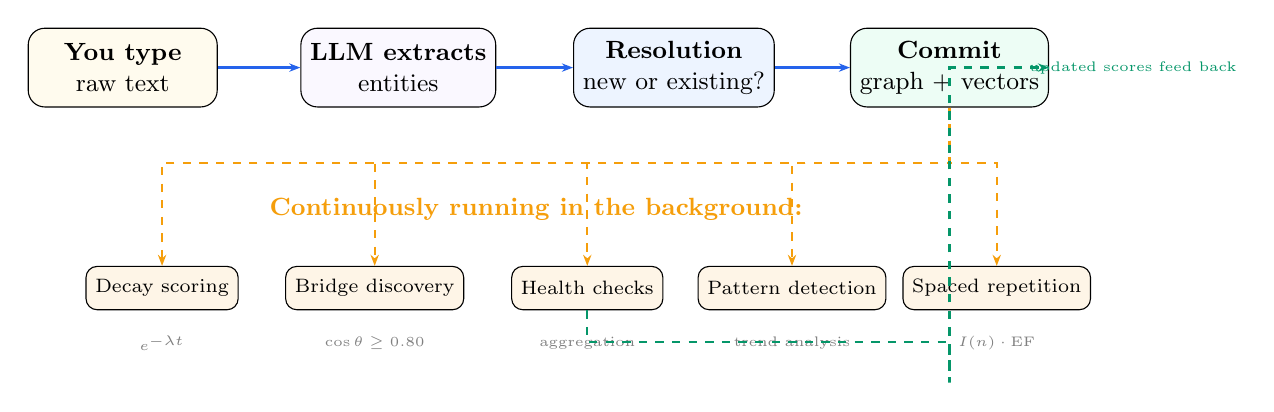
\begin{tikzpicture}[
    >={Stealth[length=4pt]},
    stage/.style={draw, rounded corners=6pt, fill=#1, minimum width=2.4cm, minimum height=1cm, align=center, font=\small},
    bgjob/.style={draw, rounded corners=4pt, fill=warm!10, minimum width=1.8cm, minimum height=0.55cm, align=center, font=\scriptsize},
]
    % Main pipeline
    \node[stage=nodeevent!30] (input) at (0, 0) {\textbf{You type}\\raw text};
    \node[stage=nodenote!30] (extract) at (3.5, 0) {\textbf{LLM extracts}\\entities};
    \node[stage=nodeperson!50] (resolve) at (7, 0) {\textbf{Resolution}\\new or existing?};
    \node[stage=nodeproject!40] (commit) at (10.5, 0) {\textbf{Commit}\\graph + vectors};

    \draw[->, very thick, accent] (input) -- (extract);
    \draw[->, very thick, accent] (extract) -- (resolve);
    \draw[->, very thick, accent] (resolve) -- (commit);

    % Background label
    \node[font=\small\bfseries\color{warm}] at (5.25, -1.8) {Continuously running in the background:};

    % Background jobs
    \node[bgjob] (j1) at (0.5, -2.8) {Decay scoring};
    \node[bgjob] (j2) at (3.2, -2.8) {Bridge discovery};
    \node[bgjob] (j3) at (5.9, -2.8) {Health checks};
    \node[bgjob] (j4) at (8.5, -2.8) {Pattern detection};
    \node[bgjob] (j5) at (11.1, -2.8) {Spaced repetition};

    % Connection lines
    \draw[->, thick, warm, dashed] (commit.south) -- ++(0,-0.7) -| (j1.north);
    \draw[->, thick, warm, dashed] (commit.south) -- ++(0,-0.7) -| (j2.north);
    \draw[->, thick, warm, dashed] (commit.south) -- ++(0,-0.7) -| (j3.north);
    \draw[->, thick, warm, dashed] (commit.south) -- ++(0,-0.7) -| (j4.north);
    \draw[->, thick, warm, dashed] (commit.south) -- ++(0,-0.7) -| (j5.north);

    % Math labels
    \node[font=\tiny\color{gray}] at (0.5, -3.5) {$e^{-\lambda t}$};
    \node[font=\tiny\color{gray}] at (3.2, -3.5) {$\cos\theta \geq 0.80$};
    \node[font=\tiny\color{gray}] at (5.9, -3.5) {aggregation};
    \node[font=\tiny\color{gray}] at (8.5, -3.5) {trend analysis};
    \node[font=\tiny\color{gray}] at (11.1, -3.5) {$I(n) \cdot \text{EF}$};

    % Feedback
    \draw[->, thick, accent3, dashed] (j3.south) -- ++(0,-0.4) -| (10.5,-4.0) |- node[right, font=\tiny\color{accent3}, pos=0.85] {updated scores feed back} (commit.east);

\end{tikzpicture}%
}
\end{center}

The pipeline runs when you type something. The background jobs run \emph{all the time}---even when you're not capturing anything, the graph is reshaping decay scores, discovering bridges between networks, detecting behavioural patterns, and scheduling reviews. The graph is alive.

%==============================================================
\section{The Point}
%==============================================================

\begin{keyidea}
\textbf{You already have the math.} Cosine similarity is the MAT223 dot product. Decay is the MAT137 exponential. The graph is the CSC148 tree, generalised. Entity resolution is a weighted sum. Spaced repetition is a geometric sequence. Bridge discovery is finding small angles between vectors.

None of these ideas require graduate-level knowledge. They require \textbf{combining} things you already understand and thinking carefully about what properties you need.

The real lesson from MAT137 was never about computing integrals. It was about asking: \textit{What exactly do I mean by this? What properties must it have? What happens at the edge cases?} That's the thinking that turns six simple ideas into a system that actually works.
\end{keyidea}

\end{document}
